\section{Finding 6 - Vulnerable OpenSSH Version}
\hrule

\begin{table}[htb]
    \renewcommand{\arraystretch}{1.5}
    \begin{tabular*}{\textwidth}{|>{\columncolor{orange!15}}p{3cm}|p{17.2cm}|}
    \textbf{Finding} & \textbf{Vulnerable OpenSSH Version}\\
    Risk& Medium\\
    Category& Vulnerable Software Version\\
    Impact& An attacker who can access the socket of the forwarding agent remotely may be able to execute unauthorized code with the same privileges as the process or cause a \ac{DoS} situation. An Attacker can perform privilege escalation when AuthorizedKeysCommand/AuthorizedPrincipalsCommand are configured.
    CVE-2021-28041, CVE-2021-41617\\\\ 
    Description&
    An nmap scan illustrated the openssh version. 
    \newline
    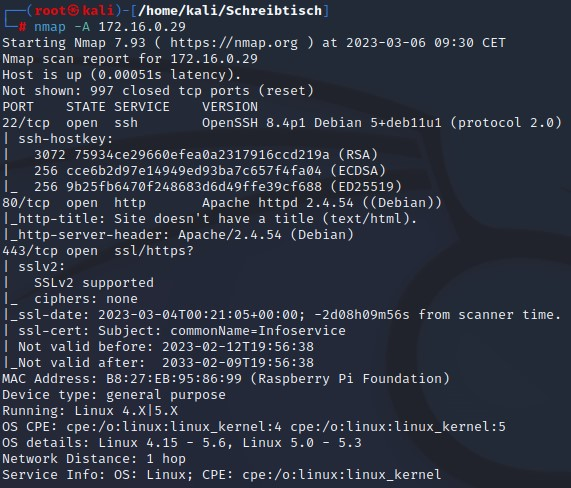
\includegraphics[width=0.73\textwidth]{vulnerable_software.jpg} 
    \newline  
    The openssh version ''OpenSSH 8.4p1 Debian 5+deb11u1 (protocol 2.0)'' has several vulnerabilites under certain circumstances mentioned in the impact part.
	\\ 
	&\\
	&\\ 
    &\\ 
    Recommendation&\\    
    \end{tabular*}
    \end{table}